\chapter{付録B NMFのモデルエビデンス}
NMFの基底数を決める際にブートストラップから計算されたモデルエビデンスを用いることを考える.
BICは最尤推定量の尤度からモデルエビデンスを近似して扱っている.
モデルエビデンスはブートストラップ法によっても近似計算できると考えられる.

基底数$k$のNMFのモデルを$\mathcal{M}_k$とおく.
ノイズ行列$H$の各要素が正規分布$\mathcal{N} (0, \sigma^2)$に従う$\mathcal{M}_k$の尤度は以下である:
\begin{align}
	p(X | Y_k, \mathcal{M}_k) = \prod_{i,j} \frac{1}{\sqrt{2 \pi \sigma^2}} \exp(-\frac{([Y_k]_{ij} - x_{ij})^2}{2 \sigma^2}).
	\label{eq:likelihood}
\end{align}
ただし,$Y_k = D_k C_k$で,$Y_k$はモデル$\mathcal{M}_k$における推定量である.
対数尤度は以下のようになる.
\begin{align}
	\log p(X | Y_k, \mathcal{M}_k) = - \frac{IJ}{2} (\log 2\pi + 2 \log \sigma) - \frac{1}{2 \sigma^2} \sum_{ij}([Y_k]_{ij} - x_{ij})^2.
\end{align}

今回の問題をBayesian model averagingの枠組みに当てはめると,異なる基底数のNMFから求まった$\bar{A}$をモデルの事後確率で重み付て足し合わせることになる.
この時の式は,
\begin{align}
	p(\bar{A}|X) = \sum_k p(\bar{A}|\mathcal{M}_k, X) p(\mathcal{M}_k | X),
\end{align}
で$p(\bar{A}|X)$を求めることになる.

モデルの事後確率は
\begin{align}
	p(\mathcal{M}_k|X) = \frac{m_k p(\mathcal{M}_k)}{\sum_l m_l p(M_l)},
\end{align}
で表される.
ただし,
\begin{align}
	m_k = \int p(X | Y_k, \mathcal{M}_k) p(Y_k| \mathcal{M}_k) dY_k,
	\label{eq:evidence}
\end{align}
である.
これはモデルエビデンスやmarginal likelihoodと呼ばれる.
また,$p(\mathcal{M}_k)$はモデルが正しい確率である.

ある条件下で,母数の事後確率の密度関数はブートストラップによる最尤推定量の分布と同じになる.
そのため,ブートストラップサンプルから推定した$Y_k$の分布をもとに事後確率を計算すれば良い.

現在は$p(\mathcal{M}_k)$に関する知識はなく無情報なため,モデルエビデンスを推定することで各モデルの重みが求まる.

\section{ラプラス近似}
モデルエビデンスの計算には事前分布を決めなければならず,積分も計算しなければいけない.
そこでラプラス近似により$m_k$は以下のような$\hat{m_k}$で近似できる.
\begin{align}
	\log \hat{m}_k = \log p(X | \hat{Y_k}, \mathcal{M}_k) - \frac{d_k}{2} \log n.
	\label{eq:simm}
\end{align}
ここで,$d_k$は母数の数($I \times K + K \times J$),$n$は観測データ数($J$)である.
この近似を使ってBayes因子のログをとったものがBICである.
Bayes因子は2つのモデルエビデンスの比である.
NMFではデータの増加とともにパラメータ数も増加するため,BICを用いて基底数を決めるのは本来適さない.

実験では,$\log p(X | \hat{Y_k}, \mathcal{M}_k)$は初期値を変えてNMFを行い,尤度が最も大きくなった対数尤度を用いる.
また,$\sigma^2 = Var(X - Y_k)$として計算する.

\section{ブートストラップによる近似}
ブートストラップの推定量の分布は最尤推定量の分布を近似する(ブートストラップサンプルが生成されたパラメータ分バイアスは乗る).
これを簡単なデモンストレーションで確認する.

人工的に$D$と$C$を作成し,標準正規分布に従うノイズを加えて$X$を作る.
事後確率$p(\mathcal{M}_k | X)$は
\begin{align}
	p(\mathcal{M}_k | X) &= \frac{p(X | Y_k, \mathcal{M}_k) p(\mathcal{M}_k)}{p(X)},
\end{align}
である.
事前分布$p(\mathcal{M}_k)$を無情報とした時,事後確率は尤度に比例する.
そこで,データ$X$のある2要素$(i,j)$と$(i',j')$について尤度の分布を図示する.
ノイズに標準正規分布を用いたので,$\sigma = 1$として\eqref{eq:likelihood}を2つの要素のある範囲について計算する.
求めたいのは事後確率の分布なので,「$[Y_k]_{ij}=5$かつ$[Y_k]_{i'j'}=8$の時の尤度を計算する」ことを5や8の値をずらしながら行う.
その結果を\Figref{fig:posprob}に示す.
\begin{figure}[htbp]
    \begin{minipage}{0.5\hsize}
			\begin{center}
					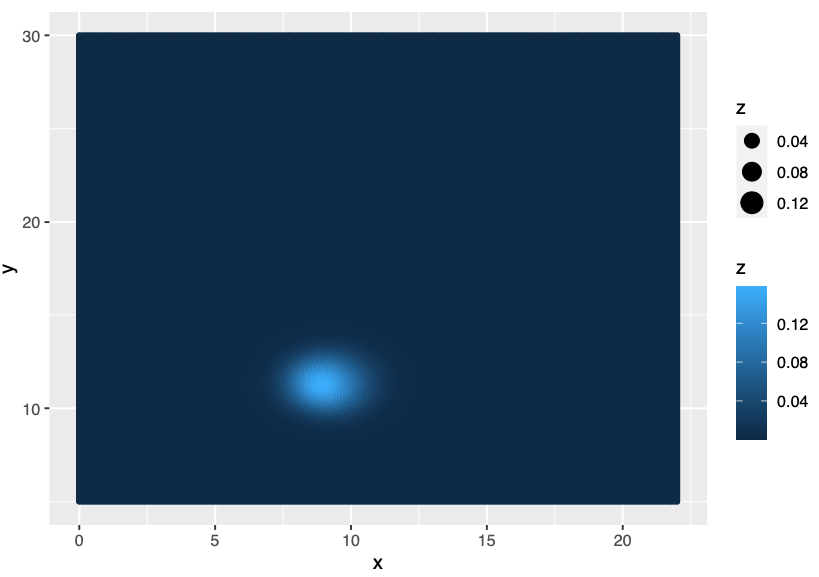
\includegraphics[width=\hsize]{posterior_prob}
					\caption{人工データの2つの要素の尤度分布}
					\label{fig:posprob}
			\end{center}
		\end{minipage}
    \begin{minipage}{0.5\hsize}
			\begin{center}
					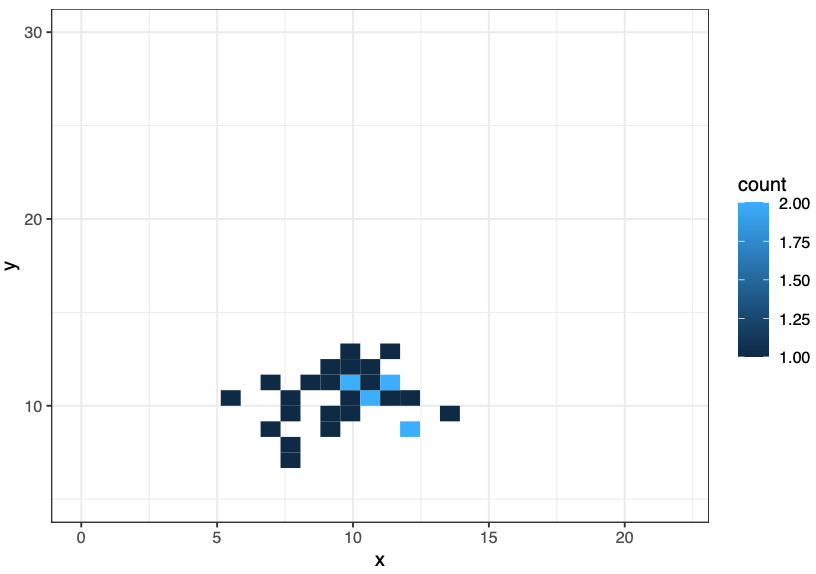
\includegraphics[width=\hsize]{boot_prob30}
					\caption{30個のブートストラップサンプルから推定された2つの要素の値の分布}
					\label{fig:boot_prob30}
			\end{center}
		\end{minipage}\\
    \begin{minipage}{0.5\hsize}
			\begin{center}
					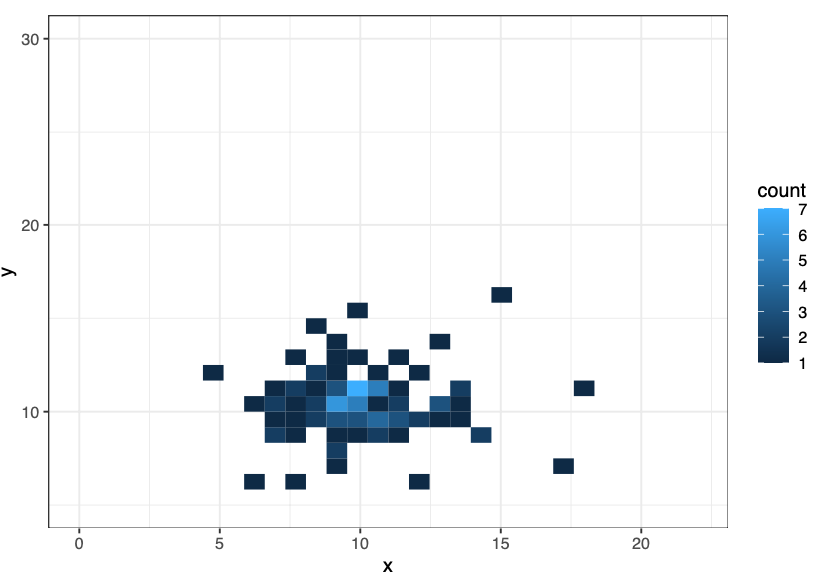
\includegraphics[width=\hsize]{boot_prob100}
					\caption{100個のブートストラップサンプルから推定された2つの要素の値の分布}
					\label{fig:boot_prob100}
			\end{center}
		\end{minipage}
    \begin{minipage}{0.5\hsize}
			\begin{center}
					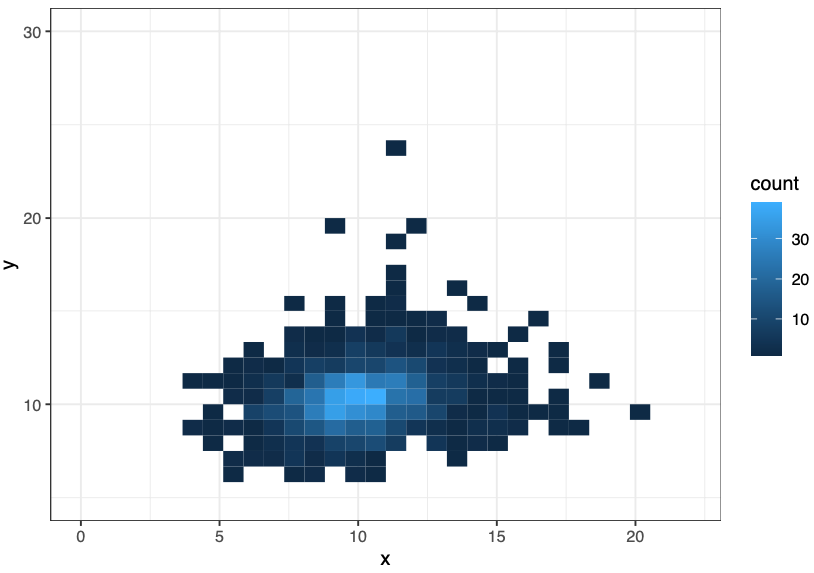
\includegraphics[width=\hsize]{boot_prob1000}
					\caption{1000個のブートストラップサンプルから推定された2つの要素の値の分布}
					\label{fig:boot_prob1000}
			\end{center}
		\end{minipage}
\end{figure}

次に,ブートストラップの推定量が\Figref{fig:posprob}を近似することを確かめる.
ブートストラップサンプルを作成しNMFを行い,\Figref{fig:posprob}の2要素についてヒートマップを作成する.
その結果をブートストラップのサンプル数別に\Figref{fig:boot_prob30}〜\ref{fig:boot_prob1000}に示す.
これより,\Figref{fig:boot_prob1000}は\Figref{fig:posprob}の分布を近似できていることがわかる.

これより,ブートストラップの推定量の分布は最尤推定量の分布を近似するので,$m_k$は以下のように近似できる.

\begin{align}
	m_k &= \int p(X | Y_k, \mathcal{M}_k) p(Y_k| \mathcal{M}_k) dY_k \\
	&\sim \frac{1}{B} \sum_b \prod_{i,j} \frac{1}{\sqrt{2 \pi \sigma^2}} \exp\left(-\frac{([Y_k^b]_{ij} - X^b_{ij})^2}{2 \sigma^2} \right).
	\label{eq:simm2}
\end{align}

ここで,$Y_k^b$はブートストラップサンプル$b$から計算された$Y_k$で,$B$はブートストラップサンプル数である.
また,$\sigma^2 = Var(X^b - Y^b_k)$として計算する.

\section{実験}
人工データセット86個について2つの近似方法でモデルエビデンスを計算した.
その結果を\Figref{fig:evidence1}と\Figref{fig:evidence2}に示す.
同じデータの結果を線で結んでいる.
ラプラス近似を行った場合は真の基底数10付近で最大値をとっている.
ブートストラップによる近似を行った場合は基底数に比例してモデルエビデンスの値も大きくなっている.
また,同じデータでも基底数によってオーダーが大きく異なるが,これは尤度計算に用いる分散をデータから計算しているためである.

\begin{figure}[htbp]
    \begin{minipage}{0.5\hsize}
			\begin{center}
					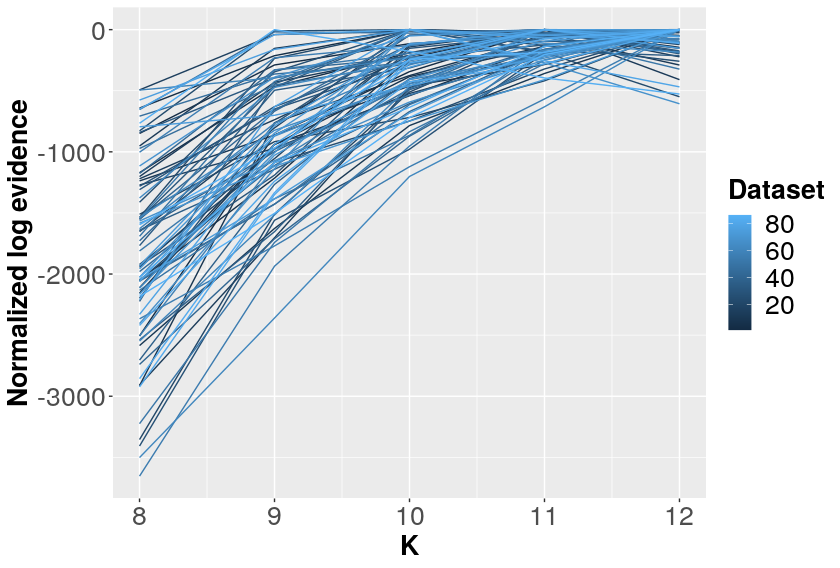
\includegraphics[width=\hsize]{evidence1log}
					\caption{ラプラス近似によって計算されたログエビデンス.各データについて最大値が0となるように定数を足した.}
					\label{fig:evidence1}
			\end{center}
		\end{minipage}
    \begin{minipage}{0.5\hsize}
			\begin{center}
					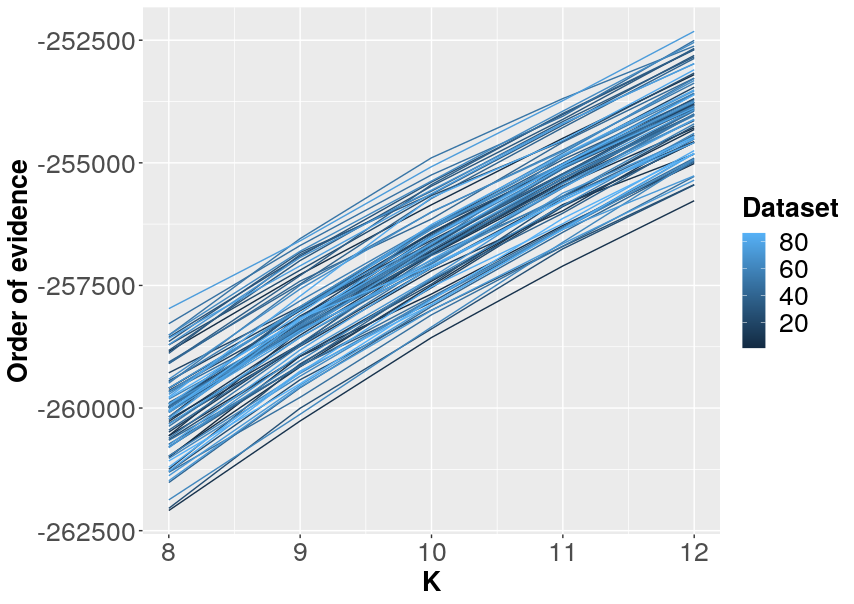
\includegraphics[width=\hsize]{evidence2order}
					\caption{ブートストラップ近似によって計算されたエビデンスのオーダー(10を底とした指数).}
					\label{fig:evidence2}
			\end{center}
		\end{minipage}
\end{figure}

また,\Figref{fig:evidence2}のログを取り,\Figref{fig:evidence1}とプロットした図を\Figref{fig:evidence12}に示す.
これより,ブートストラップによる近似を用いた場合のモデルエビデンスの値は大きいことが分かる.
ラプラス近似では$\frac{d_k}{2} \log n$というパラメータ数による補正が加わっているため,ブートストラップによるモデルエビデンスの方が高い値を持つ.
逆に,\Figref{fig:evidence12}の2つの近似手法のモデルエビデンスの差が過剰に足された補正の値だと考えることもできる.
つまり,$\frac{d_k}{2} \log n$から2つのモデルエビデンスの差を引いた数値がNMFの真の自由度であるとも考えられる.
これを確かめるためには数値実験を行う必要がある.

\begin{figure}[htbp]
    \begin{center}
        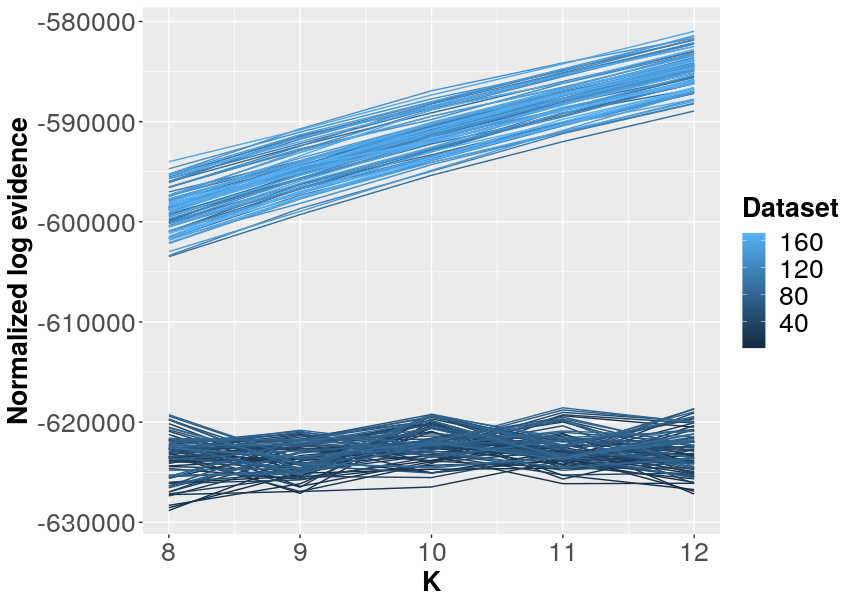
\includegraphics[width=0.8\linewidth]{evidence12log}
        \caption{2つの近似方法によって計算されたログエビデンス.}
        \label{fig:evidence12}
    \end{center}
\end{figure}
